% ============================================================
%  RESUMEN EJECUTIVO -- Álgebra Lineal Aplicada
%  Péndulo invertido sobre un carro (dos configuraciones)
%  Universidad Nacional de Colombia -- Sede Medellín
%  Mismo formato que el informe técnico; máximo 5 páginas.
% ============================================================
\documentclass[11pt,letterpaper]{article}

% ── Idioma y codificación ───────────────────────────────────
\usepackage[utf8]{inputenc}
\usepackage[T1]{fontenc}
\usepackage[spanish,provide=*]{babel}

% ── Tipografía (Palatino, look de tesis) ────────────────────
\usepackage{mathpazo}
\usepackage{microtype}
\linespread{1.02}

% ── Geometría de página ─────────────────────────────────────
\usepackage[letterpaper,top=0.9in,bottom=0.9in,left=1in,right=1in]{geometry}

% ── Matemáticas ─────────────────────────────────────────────
\usepackage{amsmath,amssymb,mathtools,bm}

% ── Color, cajas, tablas, figuras ───────────────────────────
\usepackage{xcolor}
\definecolor{acento}{RGB}{31,59,107}
\definecolor{acento2}{RGB}{120,40,40}
\usepackage[most]{tcolorbox}
\usepackage{booktabs}
\usepackage{array}
\usepackage{graphicx}

% ── Títulos de sección ──────────────────────────────────────
\usepackage{titlesec}
\titleformat{\section}
  {\normalfont\large\bfseries\color{acento}}{\thesection}{0.7em}{}
\titleformat{\subsection}
  {\normalfont\normalsize\bfseries\color{acento!85!black}}{\thesubsection}{0.6em}{}
\titlespacing*{\section}{0pt}{1.0ex plus .7ex minus .2ex}{0.5ex plus .2ex}
\titlespacing*{\subsection}{0pt}{0.8ex plus .5ex minus .2ex}{0.4ex plus .2ex}

% ── Encabezado/pie ──────────────────────────────────────────
\usepackage{fancyhdr}
\pagestyle{fancy}\fancyhf{}
\renewcommand{\headrulewidth}{0.4pt}
\fancyhead[L]{\footnotesize\itshape Resumen ejecutivo --- Péndulo invertido}
\fancyhead[R]{\footnotesize\itshape Álgebra Lineal Aplicada}
\fancyfoot[C]{\thepage}

% ── Listas y enlaces ────────────────────────────────────────
\usepackage{enumitem}
\setlist{itemsep=1.5pt,topsep=2pt}
\usepackage[colorlinks=true,linkcolor=acento,citecolor=acento2,urlcolor=acento]{hyperref}
\usepackage{cleveref}

% ── Caja para el mensaje central ────────────────────────────
\newtcolorbox{clave}[1][]{colback=acento!4,colframe=acento!55!black,
  boxrule=0.6pt,arc=2pt,left=6pt,right=6pt,top=5pt,bottom=5pt,#1}

% ── Operadores y atajos ─────────────────────────────────────
\DeclareMathOperator{\rank}{rango}
\newcommand{\R}{\mathbb{R}}
\newcommand{\xv}{\bm{x}}
\newcommand{\uv}{\bm{u}}

\crefname{table}{tabla}{tablas}\Crefname{table}{Tabla}{Tablas}
\crefname{figure}{figura}{figuras}\Crefname{figure}{Figura}{Figuras}
\addto\captionsspanish{\renewcommand{\tablename}{Tabla}}

\graphicspath{{../resumen_tecnico/figs/}}

% ============================================================
\begin{document}

% ── Cabecera ────────────────────────────────────────────────
\begin{center}
    {\footnotesize\bfseries\color{acento2} RESUMEN EJECUTIVO}\\[0.4em]
    {\LARGE\bfseries Análisis y Control del Péndulo Invertido \\[0.15em]
     sobre un Carro mediante Álgebra Lineal Aplicada}\\[0.6em]
    {\normalsize Mateo Bedoya Rojas \quad\textbullet\quad Camilo Alejandro Patiño Osorio \quad\textbullet\quad Santiago Uribe Echavarría}\\[0.3em]
    {\footnotesize Facultad de Ciencias, Universidad Nacional de Colombia, Sede Medellín}
\end{center}
\vspace{0.2em}
\hrule height 0.6pt
\vspace{0.8em}

\noindent
\begin{clave}
\small
\textbf{Propósito.} Este documento resume de forma ejecutiva el proyecto y sirve
de guía para recorrerlo. Las deducciones, definiciones y demostraciones
completas se encuentran en el \emph{informe técnico}~\cite{tecnico}, al que se
remite en cada sección. El código y su organización se documentan en el
apéndice~C de dicho informe y en el archivo \texttt{README.md} del
repositorio.
\end{clave}

% ============================================================
\section{El problema}

El \emph{péndulo invertido sobre un carro} consiste en estabilizar un péndulo en
su posición vertical \emph{superior} ---un equilibrio inestable--- aplicando una
fuerza horizontal $u(t)$ únicamente sobre el carro. Es un banco de pruebas
clásico de la teoría de control porque reúne tres rasgos que aparecen en
problemas reales (cohetes, robots bípedos, vehículos autobalanceados):
es \emph{subactuado} (más grados de libertad que actuadores),
\emph{inestable} en lazo abierto y \emph{no lineal}.

Su interés para el curso es que casi todas las preguntas relevantes se responden
con álgebra lineal: la evolución de las desviaciones la da la exponencial
matricial $e^{At}$; la estabilidad, los eigenvalores de $A$; la posibilidad de
controlar u observar, el \emph{rango} de ciertas matrices; y el diseño del
control, la reubicación de eigenvalores. Se estudian dos configuraciones de
complejidad creciente:

\begin{itemize}
  \item \textbf{Configuración I --- péndulo simple.} Una barra articulada al
  carro; estado en $\R^4$, un único modo inestable.
  \item \textbf{Configuración II --- péndulo doble.} Dos eslabones en serie;
  estado en $\R^6$, dos modos inestables. Muestra que el mismo razonamiento
  escala sin cambios conceptuales, solo con matrices mayores.
\end{itemize}

\noindent\emph{Detalle completo: informe técnico~\cite{tecnico}, Sección~1.}

% ============================================================
\section{Metodología y desarrollo}

El trabajo sigue una cadena única, idéntica para ambas configuraciones, que va
del modelo físico al controlador verificado:

\begin{enumerate}
  \item \textbf{Modelo no lineal.} Se deducen las ecuaciones de movimiento por
  el formalismo de Euler--Lagrange, obteniendo $\dot\xv=f(\xv,u)$
  (informe técnico, Sección~2).
  \item \textbf{Linealización.} Por desarrollo de Taylor de primer orden
  alrededor del equilibrio erguido se llega a la representación en espacio de
  estados $\dot\xv = A\xv + B\uv$, $\bm y = C\xv$ (Sección~2).
  \item \textbf{Análisis espectral.} Los eigenvalores de $A$ deciden la
  estabilidad; un eigenvalor con parte real positiva es la firma de la
  inestabilidad (Sección~3.1--3.3).
  \item \textbf{Controlabilidad y observabilidad.} Se aplican los criterios de
  rango de Kalman sobre las matrices $\mathcal{C}$ y $\mathcal{O}$
  (Sección~3.5--3.6).
  \item \textbf{Diseño del control.} Se calcula la ganancia $K$ de la
  realimentación $\uv=-K\xv$ por dos vías: \emph{LQR} (resolviendo la ecuación
  de Riccati vía la matriz hamiltoniana) y \emph{asignación de polos}
  (fórmula de Ackermann) (Sección~3.7--3.8).
  \item \textbf{Verificación.} Se integra el modelo \emph{no lineal} en lazo
  cerrado con $\uv=-K\xv$ y se comprueba que estabiliza partiendo de una
  pequeña inclinación (Sección~4).
\end{enumerate}

\noindent\emph{Las definiciones, teoremas y demostraciones de cada paso están en
el informe técnico~\cite{tecnico}, Secciones~2 y~3.}

% ============================================================
\section{Qué resolvimos y resultados}

El procedimiento respondió, para las dos configuraciones, las preguntas centrales
del problema: \emph{(i)} ¿es inestable?, \emph{(ii)} ¿se puede controlar con la
sola fuerza del carro?, \emph{(iii)} ¿se puede reconstruir el estado a partir de
pocas mediciones?, y \emph{(iv)} ¿cómo diseñar y validar el controlador? La
\cref{tab:exec} reúne los resultados.

\begin{table}[htbp]
  \centering
  \small
  \caption{Resultados clave (parámetros del informe técnico). El tiempo de
  asentamiento $t_s$ usa el umbral $|\theta|<0.02$~rad $\approx1.1^\circ$.}
  \label{tab:exec}
  \begin{tabular}{@{}lcccccc@{}}
    \toprule
    \textbf{Config.} & $n$ & \textbf{modos inest.} & $\rank\mathcal{C}$ & $\rank\mathcal{O}$ & $t_s$ & $\max|u|$\\
    \midrule
    Simple & 4 & 1 & 4 & 4 & 1.45 s & 6.8 N\\
    Doble  & 6 & 2 & 6 & 6 & 1.77 s & 4.2 N\\
    \bottomrule
  \end{tabular}
\end{table}

\textbf{Inestabilidad.} El espectro de lazo abierto confirma la inestabilidad:
$\sigma(A)=\{+4.21,\,0,\,-0.077,\,-4.23\}$ en el simple (un modo) y
$\{\pm8.57,\,\pm4.09,\,0,\,0\}$ en el doble (dos modos).

\textbf{Controlabilidad y observabilidad.} Ambos sistemas son completamente
controlables y observables ($\rank\mathcal{C}=\rank\mathcal{O}=n$), de modo que
el espectro puede reubicarse por realimentación y el estado reconstruirse desde
las mediciones de posición y ángulos.

\textbf{Control y verificación.} Los controladores LQR y Ackermann vuelven la
matriz de lazo cerrado $A-BK$ de Hurwitz (todos los polos con parte real
negativa). Simulando el modelo \emph{no lineal} en lazo cerrado, ambas
configuraciones se estabilizan ($|\theta|<0.02$~rad de la vertical) en menos de
dos segundos (\cref{tab:exec}). La
\cref{fig:exec} muestra la respuesta del péndulo simple: sin control el ángulo
diverge, con LQR retorna a la vertical con esfuerzo de control moderado.

\begin{figure}[htbp]
  \centering
  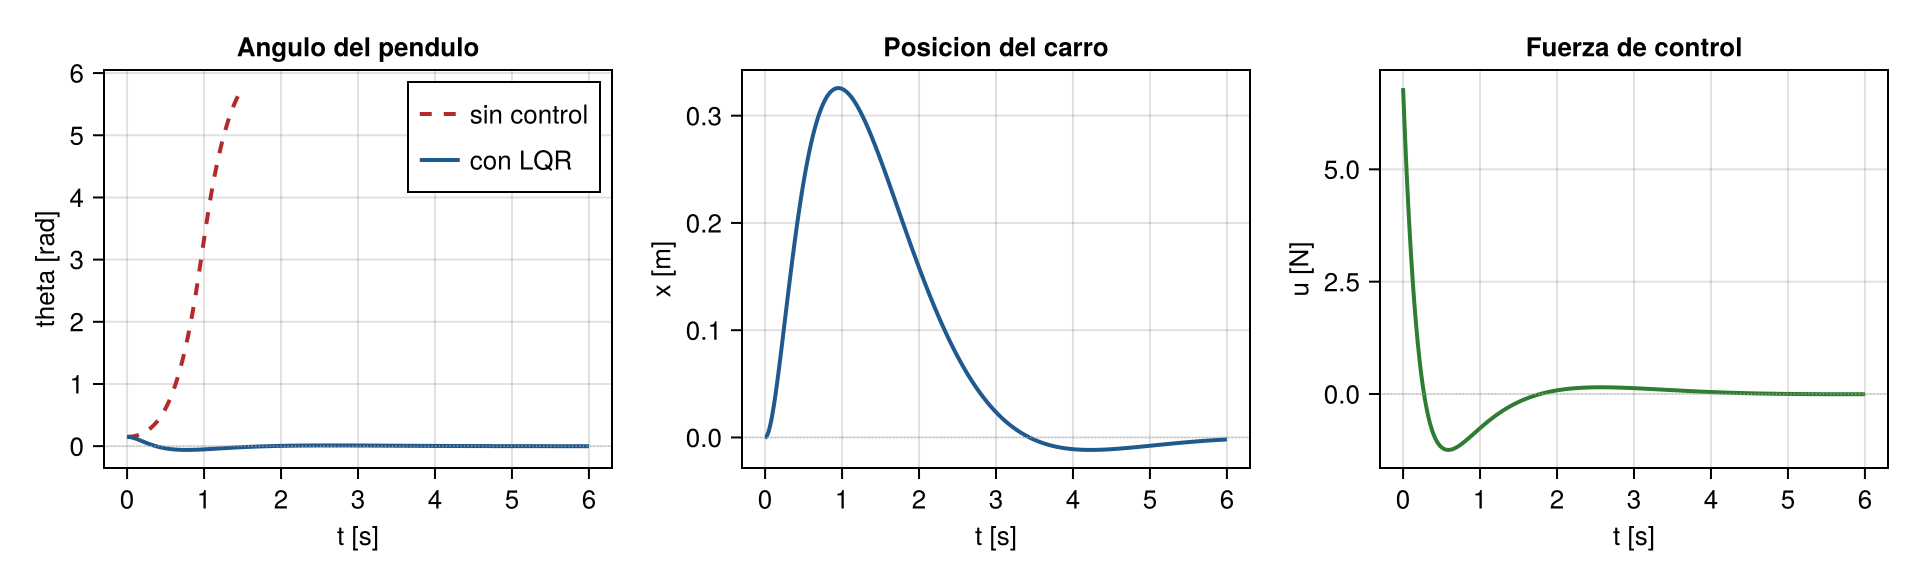
\includegraphics[width=\linewidth]{simple_respuesta.png}
  \caption{Respuesta temporal en lazo cerrado del péndulo simple (LQR),
  $\theta_0=0.15$~rad. Las respuestas del péndulo doble y la comparación
  LQR--Ackermann están en el informe técnico~\cite{tecnico}, Sección~5.}
  \label{fig:exec}
\end{figure}

\noindent\emph{Tablas y figuras completas (ganancias $K$, polos de lazo cerrado,
respuesta del doble): informe técnico~\cite{tecnico}, Sección~5.}

% ============================================================
\section{Cómo se llevó a cabo (implementación)}

Todo el análisis se implementó en \textbf{Julia} y se ejecuta de principio a fin:
los valores de la \cref{tab:exec} y las figuras se \emph{generan} corriendo el
código, no se transcriben. Las rutinas de álgebra lineal centrales
(linealización, ecuación de Riccati, fórmula de Ackermann) se programaron a
partir de las definiciones del informe, lo que hace explícito el papel de cada
concepto.

El código separa la \emph{física} (un módulo por configuración) de los
\emph{algoritmos} (genéricos en la dimensión del estado), de modo que el péndulo
doble reutiliza sin cambios el análisis y el control del simple. El flujo es:

\begin{center}\small
\texttt{model} $\rightarrow$ \texttt{linearization} $\rightarrow$
\texttt{controller} $\rightarrow$ simulación no lineal $\rightarrow$ figuras.
\end{center}

Para correr el proyecto: \texttt{julia main\_simple.jl} y
\texttt{julia main\_double.jl} ejecutan los \emph{pipelines} completos; además hay
dos cuadernos interactivos en Pluto (\texttt{notebooks/}) que permiten variar los
parámetros físicos y los pesos del controlador con deslizadores y recalcular todo
en vivo. Las instrucciones detalladas están en \texttt{README.md}.

\textbf{Validación.} La linealización analítica coincide con el Jacobiano
numérico del modelo no lineal hasta $\sim10^{-11}$, y las ganancias y espectros
obtenidos reproducen exactamente los valores reportados.

\noindent\emph{Organización del código, extractos y árbol de archivos:
informe técnico~\cite{tecnico}, Apéndice~C.}

% ============================================================
\section{Conclusión}

Un puñado de conceptos de álgebra lineal ---exponencial matricial, análisis
espectral, teoría del rango y subespacios invariantes--- basta para modelar,
analizar y controlar un sistema dinámico no trivial. El proyecto lo demuestra en
dos configuraciones del péndulo invertido: ambas se diagnosticaron inestables
pero controlables y observables, y se estabilizaron con controladores diseñados
sobre el modelo lineal y verificados sobre el no lineal. El péndulo doble
evidencia que el método escala sin cambios conceptuales. Para profundizar en
cualquier punto, este resumen remite en todo momento al informe
técnico~\cite{tecnico}.

% ============================================================
\begin{thebibliography}{9}
\small
\bibitem{tecnico}
M.~Bedoya, C.~Patiño y S.~Uribe, \emph{Análisis del Péndulo Invertido sobre un
Carro mediante Álgebra Lineal Aplicada --- Informe Técnico}. Universidad Nacional
de Colombia, Sede Medellín, 2026. 

\bibitem{ogata2010}
K.~Ogata, \emph{Modern Control Engineering}, 5.\textsuperscript{a} ed.
Upper Saddle River, NJ: Prentice Hall, 2010.

\bibitem{chen1999}
C.-T.~Chen, \emph{Linear System Theory and Design}, 3.\textsuperscript{a} ed.
New York: Oxford University Press, 1999.

\bibitem{hoffman1971}
K.~Hoffman y R.~Kunze, \emph{Linear Algebra}, 2.\textsuperscript{a} ed.
Englewood Cliffs, NJ: Prentice Hall, 1971.

\bibitem{strang2016}
G.~Strang, \emph{Introduction to Linear Algebra}, 5.\textsuperscript{a} ed.
Wellesley, MA: Wellesley--Cambridge Press, 2016.

\bibitem{hirsch2004}
M.~W.~Hirsch, S.~Smale y R.~L.~Devaney, \emph{Differential Equations,
Dynamical Systems, and an Introduction to Chaos}, 2.\textsuperscript{a} ed.
San Diego: Elsevier Academic Press, 2004.

\bibitem{golub2013}
G.~H.~Golub y C.~F.~Van Loan, \emph{Matrix Computations},
4.\textsuperscript{a} ed. Baltimore: Johns Hopkins University Press, 2013.

\bibitem{notas2026}
A.~Vélez, \emph{Notas del curso: Cálculo de Variaciones}. Universidad Nacional de Colombia, Sede Medellín, 2026.

\end{thebibliography}

\end{document}
